%%%%%%%%%%%%%%%%%%%%%%%%%%%%%%%%%%%%%%%%%
% Simple Sectioned Essay Template
% LaTeX Template
%
% This template has been downloaded from:
% http://www.latextemplates.com
%
% Note:
% The \lipsum[#] commands throughout this template generate dummy text
% to fill the template out. These commands should all be removed when 
% writing essay content.
%
%%%%%%%%%%%%%%%%%%%%%%%%%%%%%%%%%%%%%%%%%

%----------------------------------------------------------------------------------------
%	PACKAGES AND OTHER DOCUMENT CONFIGURATIONS
%----------------------------------------------------------------------------------------

\documentclass[12pt]{article} % Default font size is 12pt, it can be changed here
\usepackage[english]{babel}
\usepackage[utf8]{inputenc}
\usepackage{listings}
\usepackage{color}
\usepackage{caption}
%\usepackage[dvips]{graphicx}
\usepackage{geometry} % Required to change the page size to A4
%\geometry{a4paper} % Set the page size to be A4 as opposed to the default US Letter
\usepackage{framed}
\usepackage{url}
\usepackage{graphicx} % Required for including pictures
\usepackage{natbib}
\usepackage{float} % Allows putting an [H] in \begin{figure} to specify the exact location of the figure
%\usepackage{wrapfig} % Allows in-line images such as the example fish picture
\usepackage{hyperref}

\usepackage{fancyhdr}
\pagestyle{fancy}
\fancyhf{}
\fancyhead[RO]{{Introductory Tutorial}} 
\fancyhead[LO]{Scipion}
%\fancyhead[RO]{{\leftmark}} 
\fancyfoot[LE,RO]{{ \thepage }}

%\usepackage{lipsum} % Used for inserting dummy 'Lorem ipsum' text into the template
\definecolor{grey}{rgb}{0.9,0.9,0.9}

\linespread{1.2} % Line spacing

%\setlength\parindent{0pt} % Uncomment to remove all indentation from paragraphs

\newcounter{ejercicioNo}
\begin{document}

%----------------------------------------------------------------------------------------
%	TITLE PAGE
%----------------------------------------------------------------------------------------

\begin{titlepage}

\newcommand{\HRule}{\rule{\linewidth}{0.5mm}} % Defines a new command for the horizontal lines, change thickness here

\center % Center everything on the page

\textsc{\LARGE National Center for Biotechnology}\\[1.5cm] % Name of your university/college
%\textsc{\Large Proyecto de Sistemas Informaticos}\\[0.5cm] % Major heading such as course name
%\textsc{\large Departamento de Informática}\\[0.5cm] % Minor heading such as course title
\textsc{\Large Biocomputing Unit}\\[0.5cm] % Minor heading such as course title

\HRule \\[0.4cm]
{ \huge \bfseries Introductory Tutorial}\\[0.4cm] % Title of your document
\HRule \\[1.5cm]

%\begin{minipage}{0.4\textwidth}
%\begin{flushleft}
% \large
%\emph{Author:}\\
%Roberto  \textsc{Marabini Ruiz} % Your name
%\end{flushleft}
%\end{minipage}

%\begin{minipage}{0.4\textwidth}
%\begin{flushright} \large
%\emph{Supervisor:} \\
%Dr. James \textsc{Smith} % Supervisor's Name
%\end{flushright}
%\end{minipage}\\[4cm]

%{\large \today}\\[3cm] % Date, change the \today to a set date if you want to be precise

%\includegraphics{Logo}\\[1cm] % Include a department/university logo - this will require the graphicx package

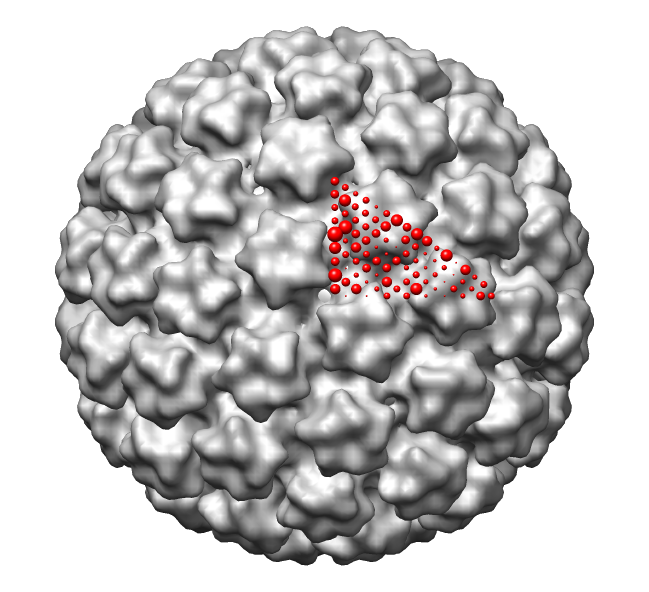
\includegraphics[width=0.75\textwidth]{{images/13.VolumeChimeraAndProjections}.png}

\vfill % Fill the rest of the page with whitespace
%\begin{minipage}{0.4\textwidth}
\begin{flushright}
 \large
%\emph{Author:}\\
  \textsc{Scipion Team} % Your name
\end{flushright}
%\end{minipage}

\end{titlepage}


%----------------------------------------------------------------------------------------
%	OBJETIVOS
%----------------------------------------------------------------------------------------



\subsection*{Intended audience}

This tutorial provides a general introduction to Scipion, an image
processing framework to obtain 3D models of macromolecular complexes
using Electron Microscopy (EM). It is designed to introduce 3D image
processing in EM to people without any prior knowledge of Scipion,
only limited knowledge about 3D-EM image processing, and with basic
computer skills.

\subsection*{We'd like to hear from you}

We have tested and verified the different steps described in this demo
to the best of our knowledge, but since our programs are in continuous
development you may find inaccuracies and errors in this text. Please,
let us know about any error you find, as well as your suggestions for
future editions by writing to
\href{mailto:scipion@cnb.csic.es}{scipion@cnb.csic.es}.

\newpage
%----------------------------------------------------------------------------------------
%	TABLE OF CONTENTS
%----------------------------------------------------------------------------------------

\tableofcontents % Include a table of contents

\newpage % Begins the essay on a new page instead of on the same page as the table of contents 


\section{General Introduction}

\subsection{Download and Install}

The first step before start working on your projects is to download and
install Scipion and all the related programs. At \href{http://scipionwiki.cnb.csic.es}{Scipion's website} 
there is all the information needed to download and install the package.

\section{Reconstruction of a viral capsid}

In this demo, we have used the single particle analysis approach to obtain
a 3D reconstruction of a {\emph Bovine Papillomavirus}. The EM images have been
collected at 300 kV and a calibrated magnification of 56,588, giving a pixel
size  of 1.237 \AA  \citep{Wolf2010}. Data have been kindly
provided by \href{http://grigoriefflab.janelia.org/}{Dr. Grigorieff’s Lab}.

\subsection{Getting started}

The data you will work on may be downloaded using the following command:

\verb+scipion testdata --download+

The data will be download in \emph {scipion\_folder/data}. After download, you must
launch the MAIN GUI by typing: \verb+scipion+

Then, create a new project by clicking \textbf{Create project} button, type a 
\textit{project name} and click OK. The GUI main project window will be launched.
The left panel contains different protocols grouped in categories. Clicking on
a group will display a menu with protocols that can be selected to launch the
corresponding GUI.

\subsection{Preprocessing}

\subsubsection{Import micrographs}

The first step is to import the micrographs to your scipion project. To do this,
press on \textbf{Import Micrographs} button. In \textit{Pattern}  you must indicate
where your micrograph files are stored (clicking on \textbf{browse} button). The 
complete pattern are:
(\emph {\$SCIPION\_HOME/data/tests/xmipp\_tutorial/micrographs/*.mrc}).

Modify the parameters of the Import Micrographs protocol according to the ones
shown in figure~\ref{ImportMics}.

\begin{figure}
\centering
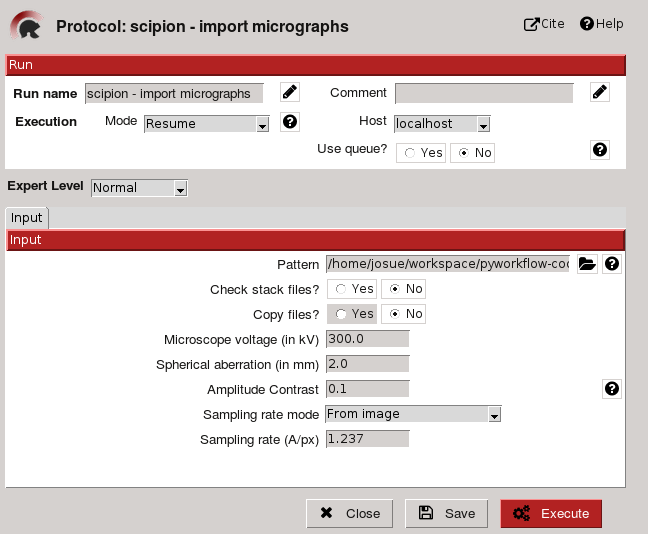
\includegraphics[width=0.75\textwidth]
{{images/01.Import_Mics}.png}
\caption{Import Micrographs protocol GUI.}
\label{ImportMics}
\end{figure}

When you have completed the form, click on the \textbf{Save \& Execute} button. After
executing the protocol, it will appear in the main Scipion project GUI the new
information shown in figure~\ref{ProjectGUI}

If we press in the \textbf{Analyze results} button it will appear a new pop-up GUI that shows
us the different imported micrographs (not shown)

\begin{figure}
\centering
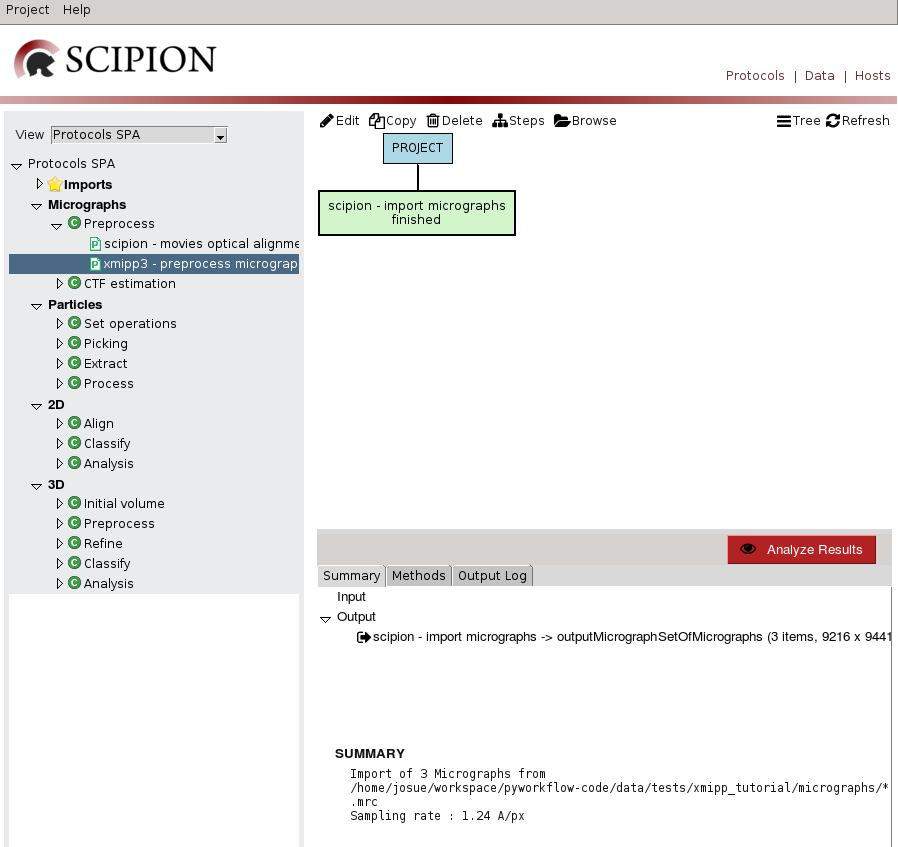
\includegraphics[width=0.9\textwidth]{{images/02.Project_GUI}.png}
\caption{Scipion project GUI after processing Import Micrograph protocol.}
\label{ProjectGUI}
\end{figure}

\subsubsection{Downsampling micrographs}

After importing the micrographs to your Scipion project, you can perform the
next processing step that consists in preprocess micrographs. This protocol
uses several xmipp programs in order to perform several operations over the
micrographs. In this example we use the options shown in figure~\ref{Preprocess}.
Please, put the values as same as figure~\ref{Preprocess}.

\begin{figure}
\centering
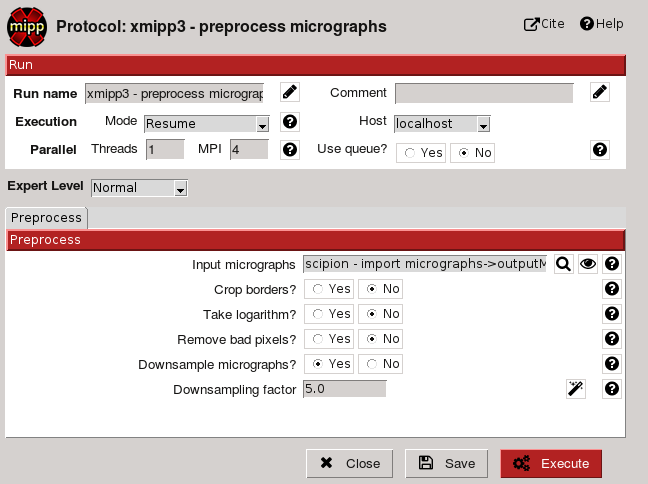
\includegraphics[width=0.75\textwidth]{{images/03.Downsampling_Mics}.png}
\caption{Preprocess Micrographs GUI.}
\label{Preprocess}
\end{figure}

\subsubsection{CTF estimation}
The next step is to estimate the CTF of the micrographs. In Scipion you can
estimate the CTF with (at the moment) CTFFind  \citep{Mindell2003} and Xmipp
CTF estimation. You don't have to do anything extra, e.g. change the extension of
the micrographs, to use both programs because in Scipion the inputs and
outputs that belongs to same type of protocols are standarized.

This protocols estimate the PSD (Power Spectrum density) of the micrographs to
estimate the parameters of the CTF (defocus U, defocus V, defocus angle, etc).
They cut the micrographs into a plenty of images with a desire size. After that,
calculate the Fourier transform to each image and averaged.

\begin{description}
\item [CTFFind:] in order to estimate the CTF with CTFFind, you will need
some parameters describing the frequency region to be analyzed. The parameters
shown in figure~\ref{CTFFind} are the adequate ones for this example.
The limit values from frequencies must be adequate so that all zeros of
the psd are contained within those frequencies. There is a wizard, shown
in figure~\ref{CTFwizard}, to choose those frequencies. The range of
defocus to search is usually larger than the ones used in this example
and according to your data set.

\item [Xmipp CTF estimation:] if you prefer, you can estimate the CTF with
Xmipp CTF estimation. The parameters used in this protocol are the same as
CTFFind protocol, explained above.

\end{description}

\begin{figure}
\minipage{0.47\textwidth}
  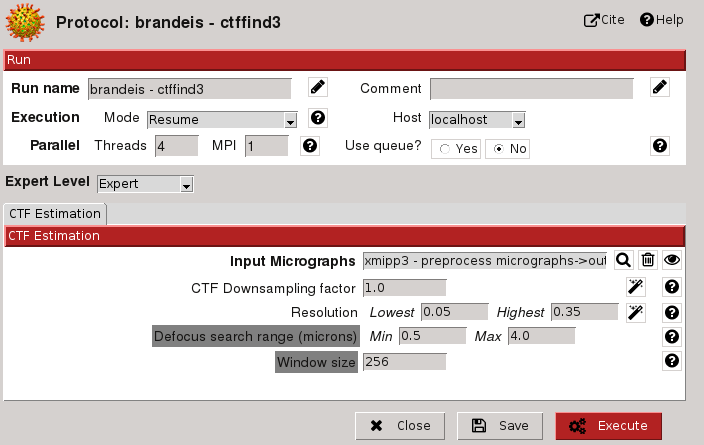
\includegraphics[width=\linewidth]{{images/04.CTFFind}.png}
  \caption{Ctffind protocol GUI}
  \label{CTFFind}
\endminipage\hfill
\minipage{0.51\textwidth}
  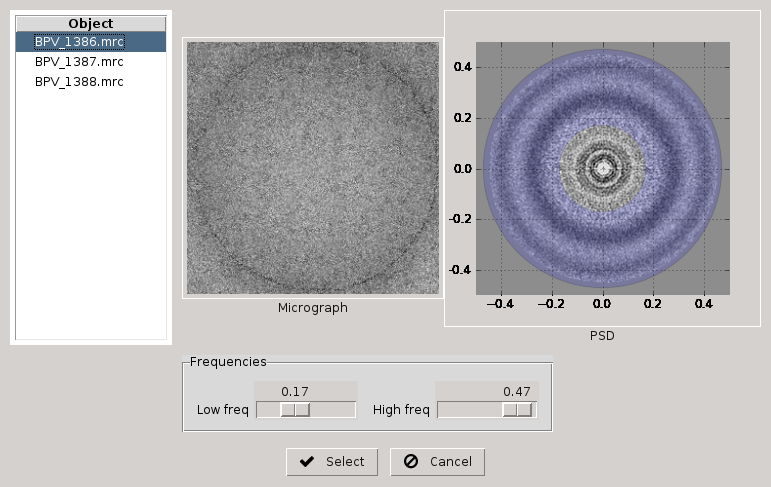
\includegraphics[width=\linewidth]{{images/16.CTFWizard}.png}
  \caption{wizard of the frequencies}
  \label{CTFwizard}
\endminipage\hfill
\end{figure}

The CTFs of good micrographs typically have multiple concentric rings, shown
in figure ~\ref{CTFs} left, extending from the image center towards its edges.
Bad micrographs may lack rings or have very few rings that hardly extend from
the image center. A reason to discard micrographs may be the presence of
strongly asymmetric rings (astigmatism, figure ~\ref{CTFs} center) or rings
that fade in a particular direction (drift, figure ~\ref{CTFs} right).

When the protocol, either CTFFind or Xmipp CTF estimation, is finished you may
click on \textbf{Analyze Result} button (figure \ref{CTFResult}). To discard
micrographs with bad CTFs you may click with the mouse right button and press
\textbf{Discard} button. Once you finish the selection, press on \textbf{Micrographs}
button (figure~\ref{CTFResult}).

Sometimes, the CTF estimation algorithm may fail to find the rings even
if they can be seen by eye. If this is the case, you may help the algorithm
to find the rings by clicking with the mouse right button and pressing
\textbf{Recalculate CTF} in the corresponding row of the Output visualization.
A graphical interface will help you to correctly identify the CTF. You must
provide the first CTF zero and the limits and press OK. When you finish, press
\textbf{Recalculate CTFs} button (figure \ref{CTFResult}).

\begin{figure}
\centering
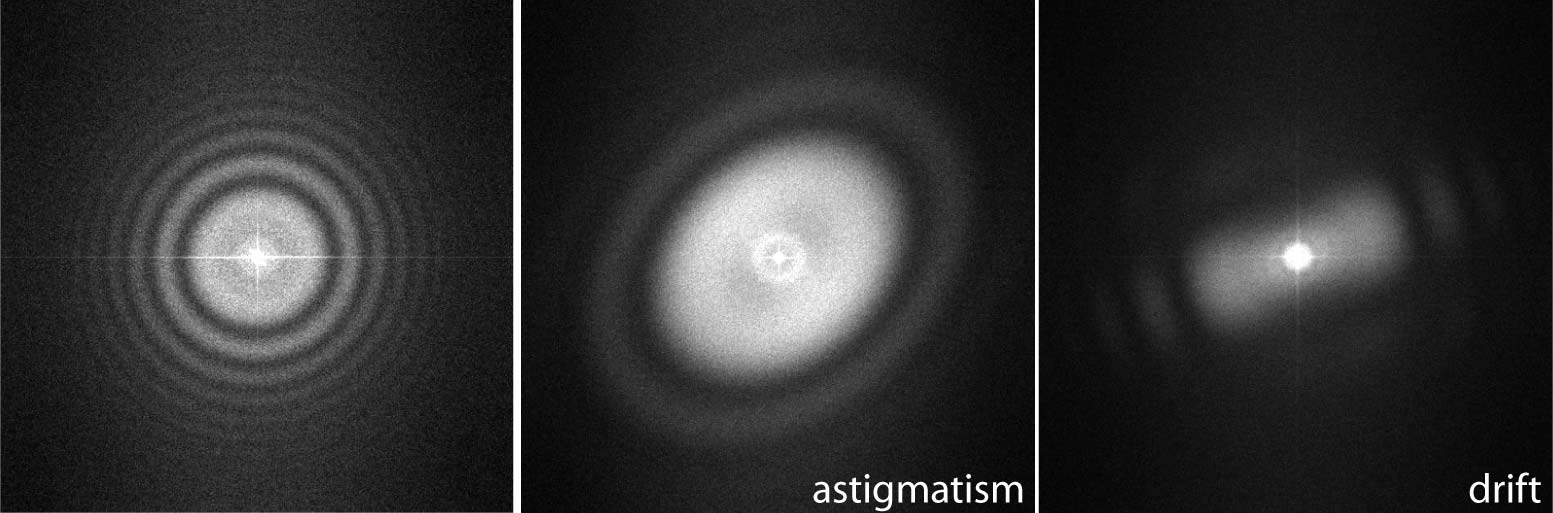
\includegraphics[width=0.75\textwidth]{images/images-016.jpg}
\caption{CTF of good, astigmatic and drift micrographs respectively}
\label{CTFs}
\end{figure}

\begin{figure}
\centering
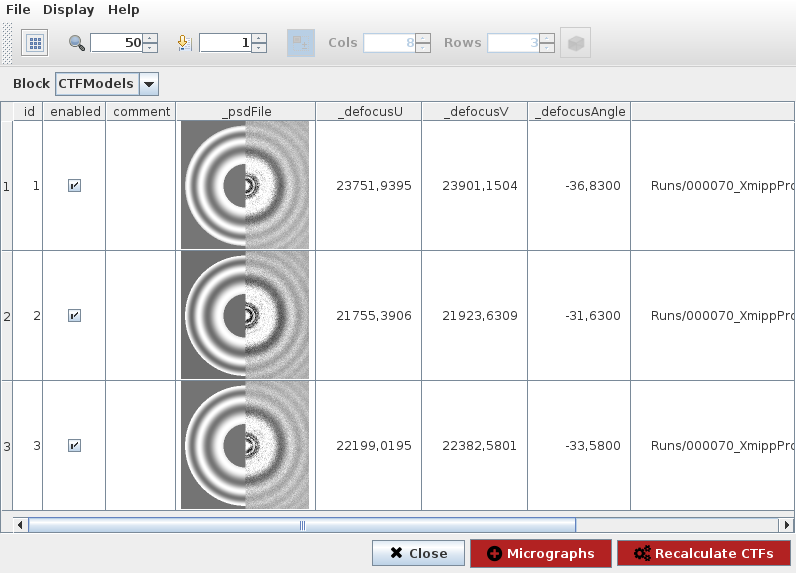
\includegraphics[width=0.75\textwidth]{{images/17.CTFREsults}.png}
\caption{Output visualization of CTFFind protocol that shows the
CTF of all the micrographs and different parameters}
\label{CTFResult}
\end{figure}

\subsubsection{Particle picking}
Now you are ready to pick the particles. You can pick the particles in the
micrographs with either Xmipp manual picking, Eman boxer or bshow protocol.
This protocols are in interactive mode, i.e: you can create different set of
coordinates in the same protocol.


\begin{description}
\item [EMAN boxer:] Click on eman2 boxer and will launch a window as shown
in figure~\ref{EmanProtocol}. Set the paramaters as shown in figure~\ref{EmanProtocol}

\begin{figure}
\centering
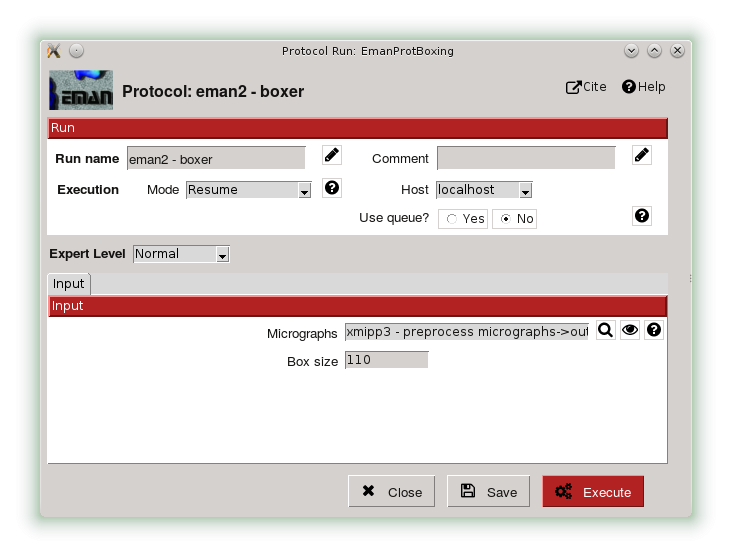
\includegraphics[width=0.75\textwidth]{{images/18.EmanPP}.png}
\caption{EMAN boxer protocol launch GUI}
\label{EmanProtocol}
\end{figure}

Once you press \textbf{Execute} button, a several windows will open
(figure~\ref{EmanPP}). This protocol has several modes of selection,
please visit it's \href{http://blake.bcm.edu/emanwiki/EMAN2}{webpage}
to futher information. When you are done picking particles press
\textbf{Done} and you will be asked if you want to create the output.
If you choose \textbf{No} you can keep picking later and selected
particles will be added to the same Set until you say \textbf{Yes}.

\begin{figure}
\centering
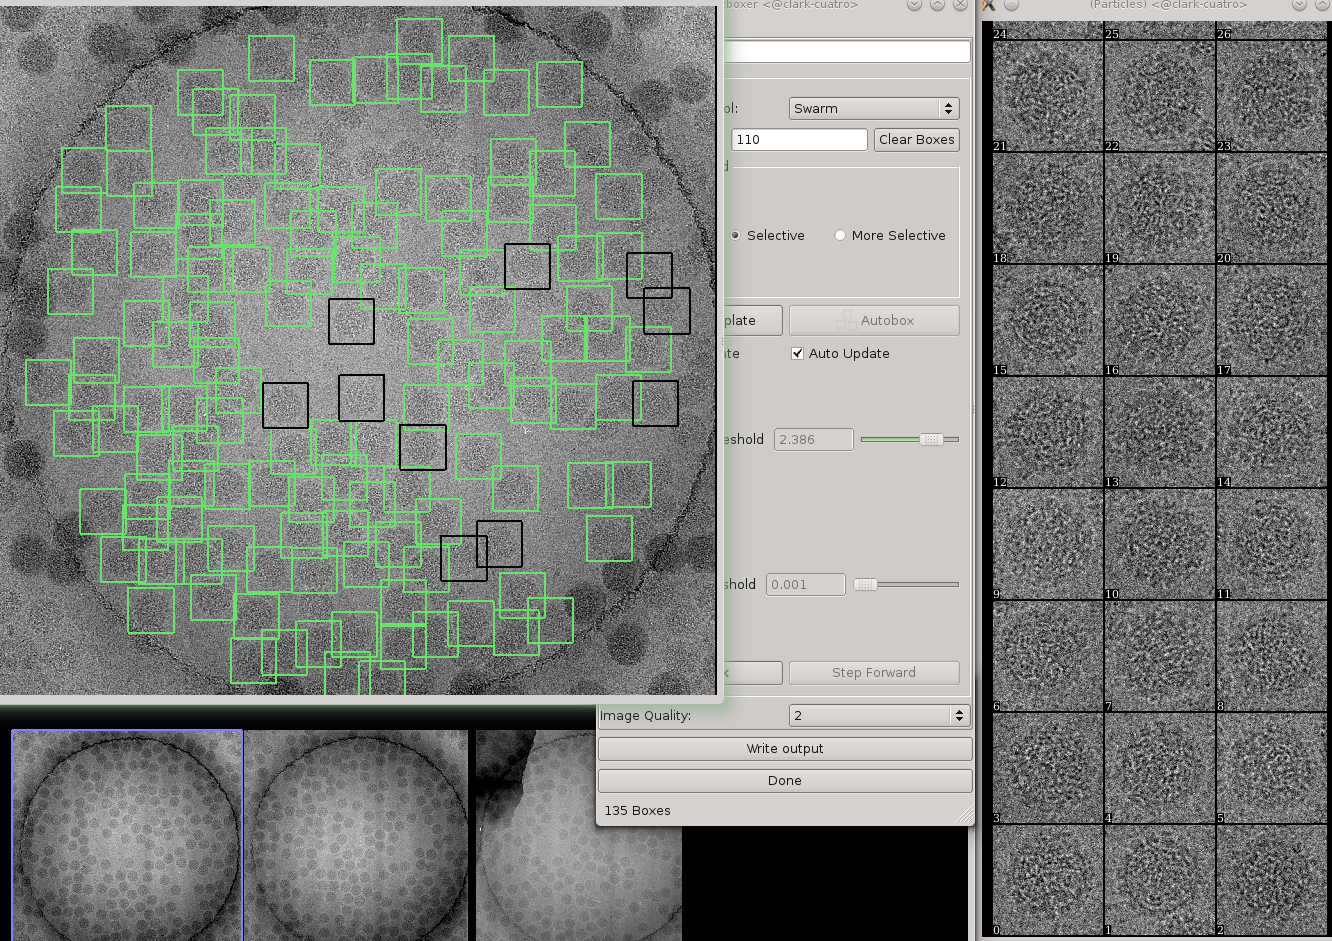
\includegraphics[width=0.75\textwidth]{{images/05.EmanPicking}.png}
\caption{GUI for EMAN boxer}
\label{EmanPP}
\end{figure}

\item [Xmipp particle picking:] If you want, click on xmipp-manual picking
protocol and will launch a window as shown in figure~\ref{XmippPP}. This
will launch a window as shown in figure~\ref{PickingParticles}

\begin{figure}
\centering
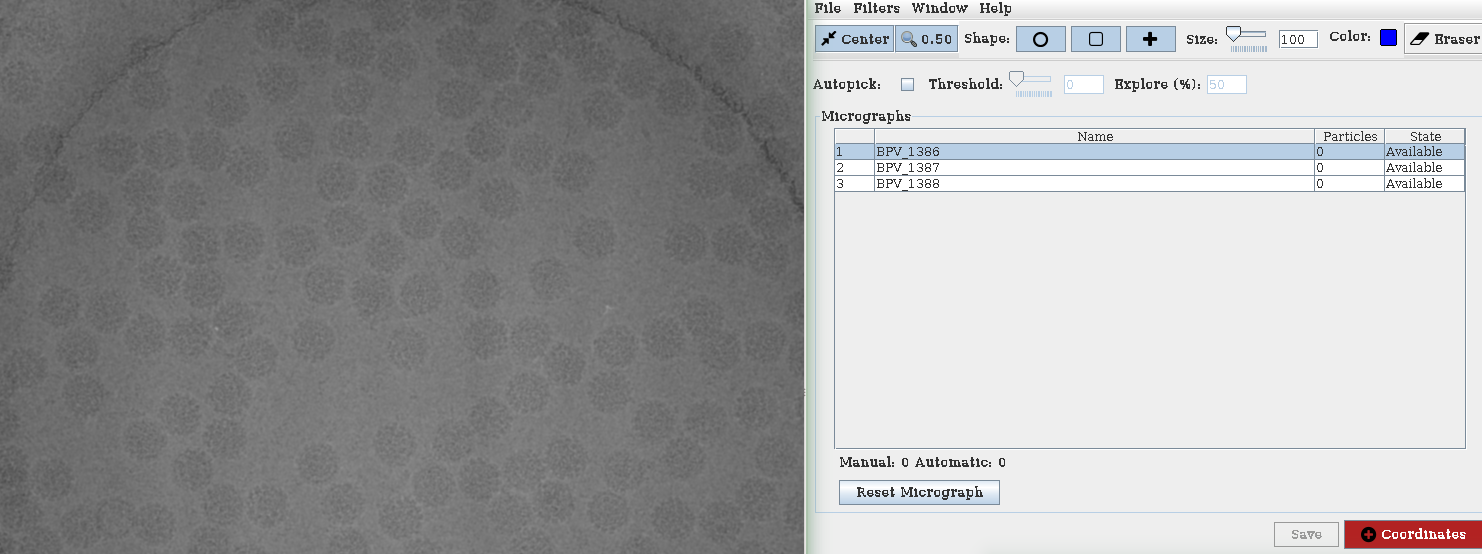
\includegraphics[width=0.75\textwidth]{{images/12-xmipp_manual_picking_protocol}.png}
\caption{GUI for Xmipp manual picking}
\label{XmippPP}
\end{figure}

\begin{figure}
\centering
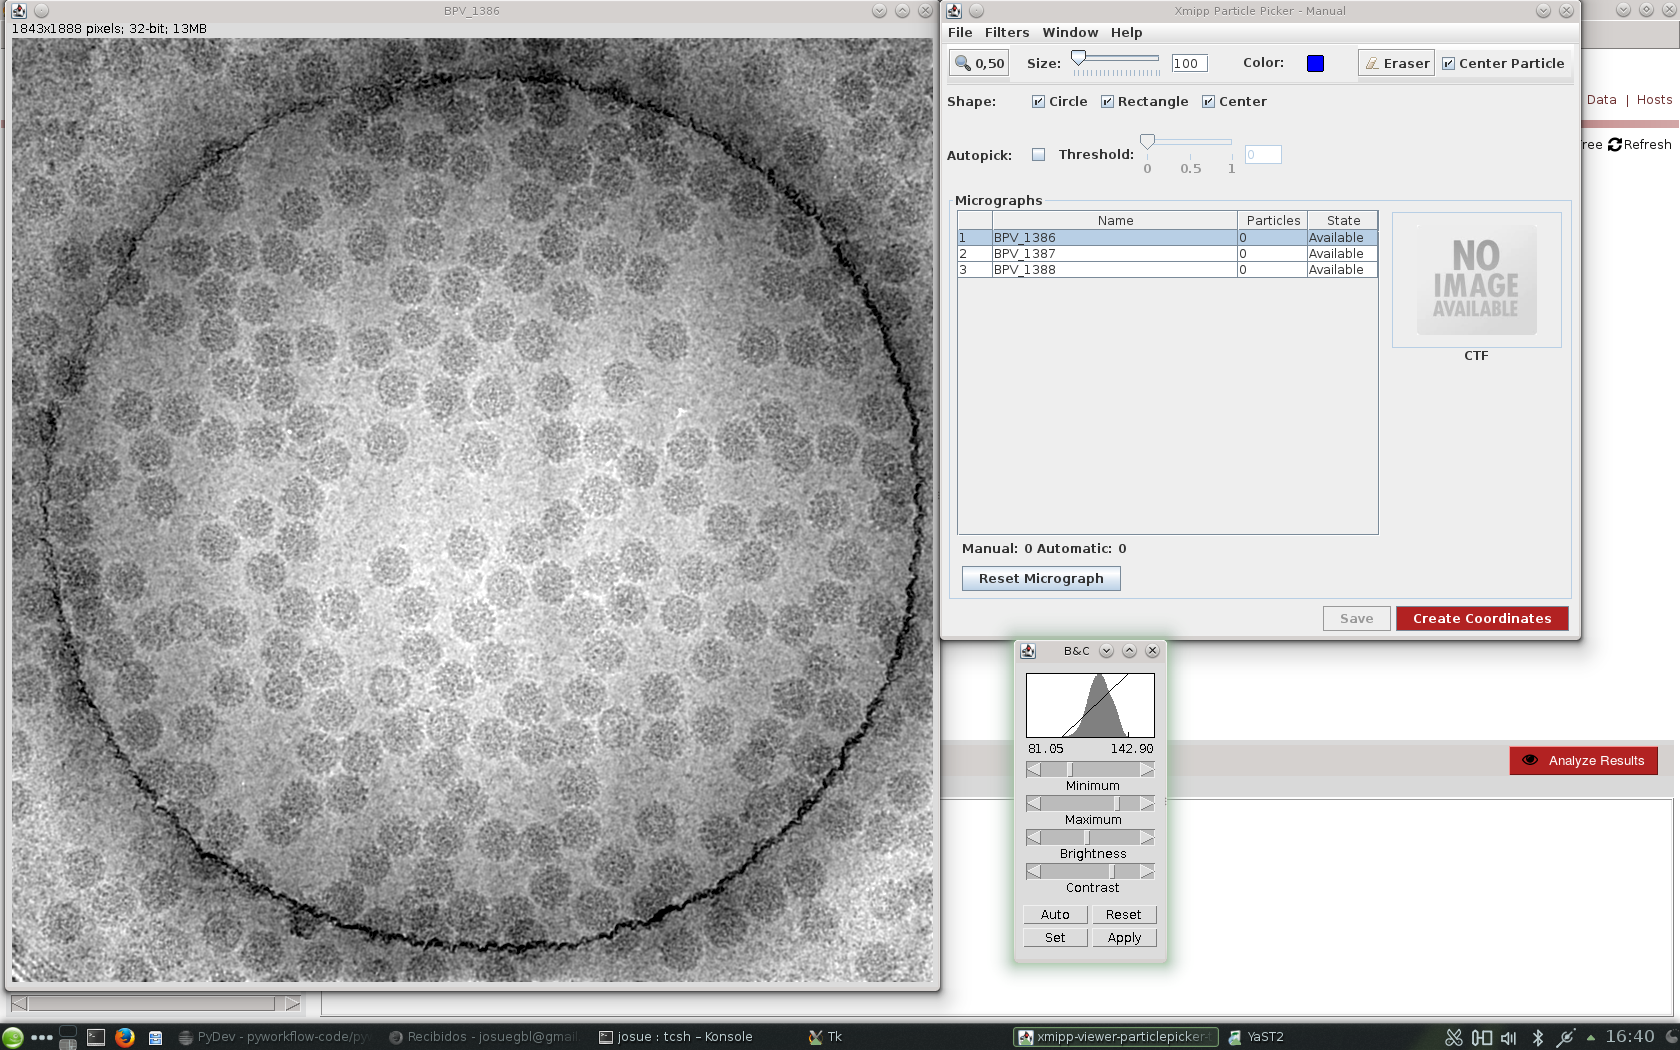
\includegraphics[width=0.75\textwidth]{{images/15.PartPickingXmipp}.png}
\caption{GUI for Xmipp Manual Particle Picking}
\label{PickingParticles}
\end{figure}

In order to select particles:

  \begin{itemize}
   \item Use Shift+Middle Mouse Button in the overview window to Zoom-in and Zoom-out.
   \item Mark particles with the left mouse button in the zoom windows. You may move
         its position by clicking the left mouse button on the selected particle and
         drag it to the new position.
   \item Use Shift+Left Mouse Button over a selected particle in order to remove it.
   \item You can apply filters to the micrographs, so that you may see the particles
         better. Filters are added into a queue, so whenever you change the visualized
         area, they are applied again. Select the menu filter in the overview window
         and add as many filters as you like.
   \item You can clean the filter queue, if you want to return to the original image
   \item You can create the set of coordinates or just save the picked particles to
         continue picking later.
  \end{itemize}

\end{description}

\subsection{Extract Particles}

 Click on Extract Particles protocol. This will launch the GUI of the next
 protocol that will allow you to extract, normalize and correct the CTF-phase
 of your picked particles, among other processes. Modify the parameters of the
 Extract Particle Protocol according to the parameters shown in figure~\ref{Extract}
 and figure~\ref{ExtractParams}.
 
 \begin{figure}
  \centering
  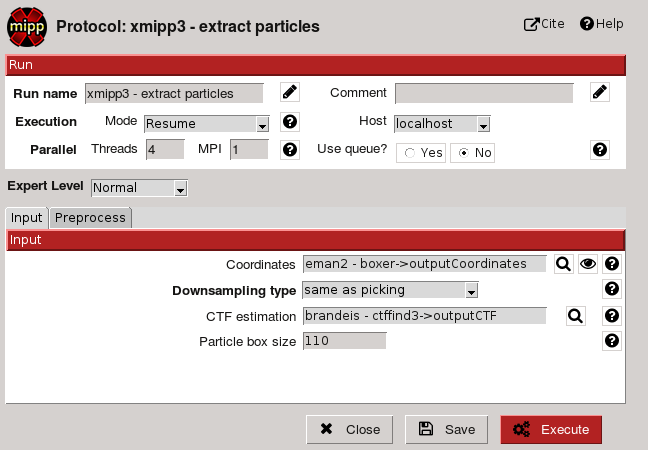
\includegraphics[width=0.75\textwidth]{{images/06.Extract_Particles}.png}
  \caption{GUI of Extract Particles protocol}
  \label{XmippPP}
 \end{figure}
 
 \begin{figure}
  \centering
  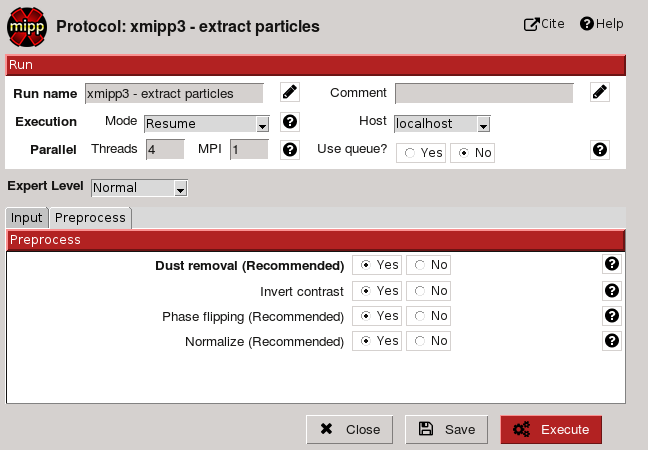
\includegraphics[width=0.75\textwidth]{{images/06.Extract_ParticlesB}.png}
  \caption{GUI of Extract Particles protocol II}
  \label{ExtractParams}
 \end{figure}
 
 \begin{itemize}
  \item The protocol extracts the particles from the micrographs using the coordinates
        determined in the previous step. You must indicate the SetOfCordinates and the
        Particle Box size in pixels (in this case 110 px).
  \item If the \textit{Normalize} flag is set to Yes (recommended), the particles are
        normalized to have zero mean and a standard deviation of unity for the
        background pixels.
  \item If the \textit{Phase flipping} is set to Yes (recommended), the protocol corrects
        the CTF-phase of your particles.
  \item If the \textit{Invert contrast} is set to Yes then bright regions become dark
        regions and the opposite. This flag should be set so that the extracted particles
        are white over a dark background.
  
 \end{itemize}
 
 The protocol also sorts the particles based on general statistics assigning to each
 particle a Zscore value. Particles with low Zscore are reliable and the ones with
 large Zscore are outliers. Press Analyse Results button in the main Scipion project
 GUI to check the extracted and normalized images.

\subsubsection{Particles selection}
By default, the visualization of the particles are sorted by zScore. If you
want to remove some particles because they are outliers, particle press
\textbf{Right} button on it and select Disable. When you have finished the
selection press \textbf{Particles} button to create a new SetOfParticles
(figure~\ref{SubsetSelection}).

 \begin{figure}
  \centering
  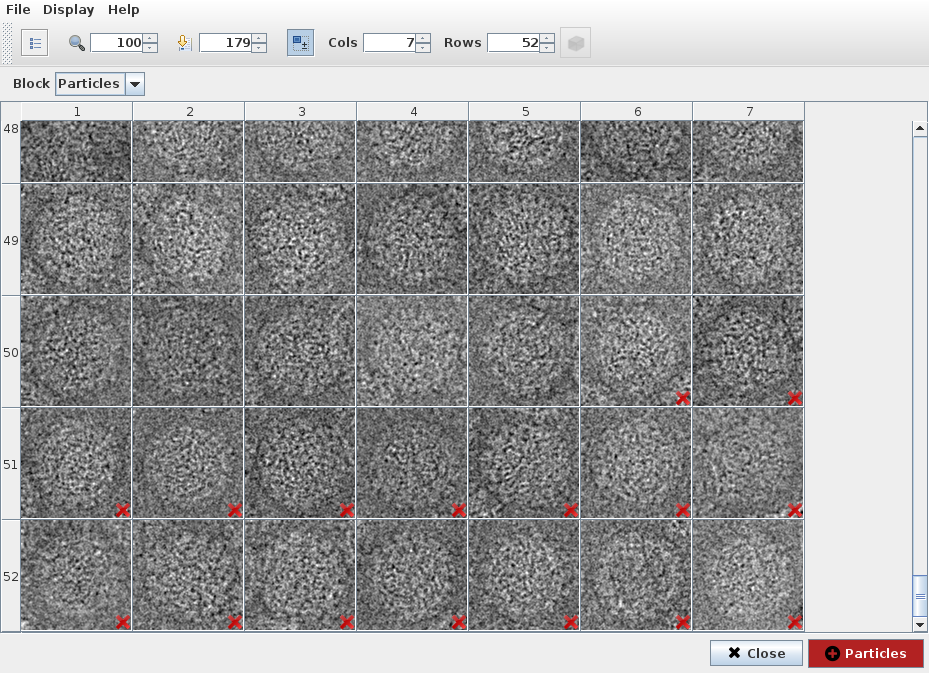
\includegraphics[width=0.75\textwidth]{{images/08.ImgsSelection}.png}
  \caption{Analyze results window of Extract Particle protocol.}
  \label{SubsetSelection}
 \end{figure}

\subsection{3D reconstruction: projection matching}

Having the right angles of each projection is crucial for making a 3D reconstruction.
However, in 3DEM you don’t know a priori the angles and you have to estimate them as
part of the problem. The most popular way of estimating them is by comparing somehow
the projections of a volume that is similar to the volume to be reconstructed
(initial model) with the images obtained from the microscope. A possible approach
consists in generating equidistant projections from the initial model. The experimental
data set is then compared (for example, by cross correlation) to each reference projection.
A “similarity” coefficient (for example, crosscorrelation coefficient) is generated
between each experimental particle and reference projection. Each individual experimental
particle is matched to the reference projection that gave the highest “similarity”
coefficient. Therefore, it is assumed that this experimental particle was projected with
the same Euler angles as the reference projection.

As is necessary an initial map, you need to import a volume. Press on \textbf{Import Volume}
and set in \textit{Pattern} parameter the following path:

\emph {\$SCIPION\_HOME/data\/tests/xmipp\_tutorial/micrographs/BPV\_scale\_filtered\_windowed\_110.vol}.

Please, set 6.185 on \textit{sampling rate} parameter.

In order to lauch the projection matching protocol click on 
\textbf{refine > projection matching} and set the parameters as
the ones shown in figures \ref{ProjMatchA}, 
\ref{ProjMatchB}, \ref{ProjMatchC} and \ref{ProjMatchD}. Choose the SetOfParticles
that has been selected previously in subset selection protocol.

 \begin{figure}
  \centering
  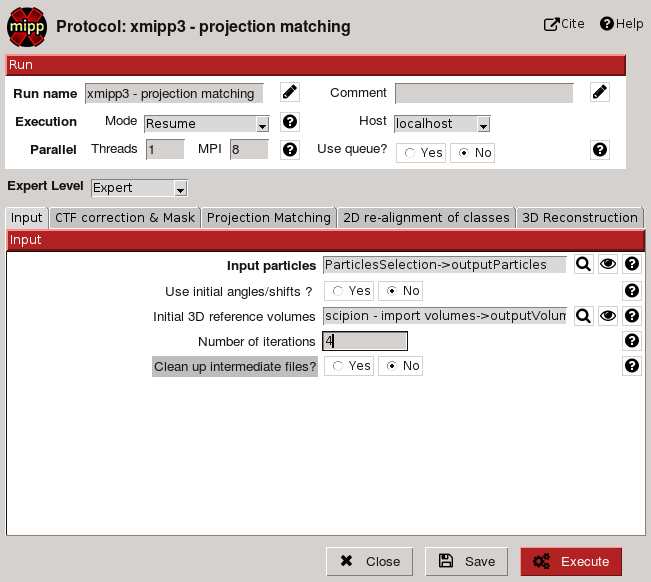
\includegraphics[width=0.75\textwidth]{{images/09.ProjMatchA}.png}
  \caption{Projection matching parameters I}
  \label{ProjMatchA}
 \end{figure}

 \begin{figure}
  \centering
  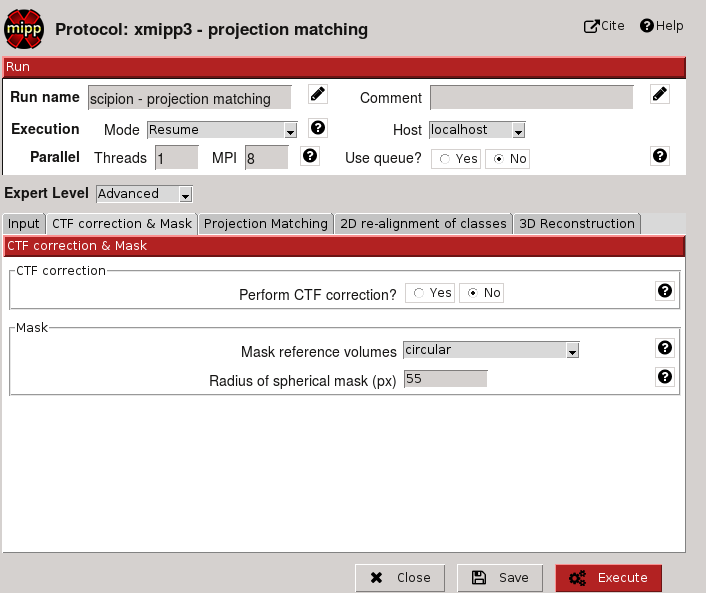
\includegraphics[width=0.75\textwidth]{{images/09.ProjMatchB}.png}
  \caption{Projection matching parameters II}
  \label{ProjMatchB}
 \end{figure}

  \begin{figure}
  \centering
  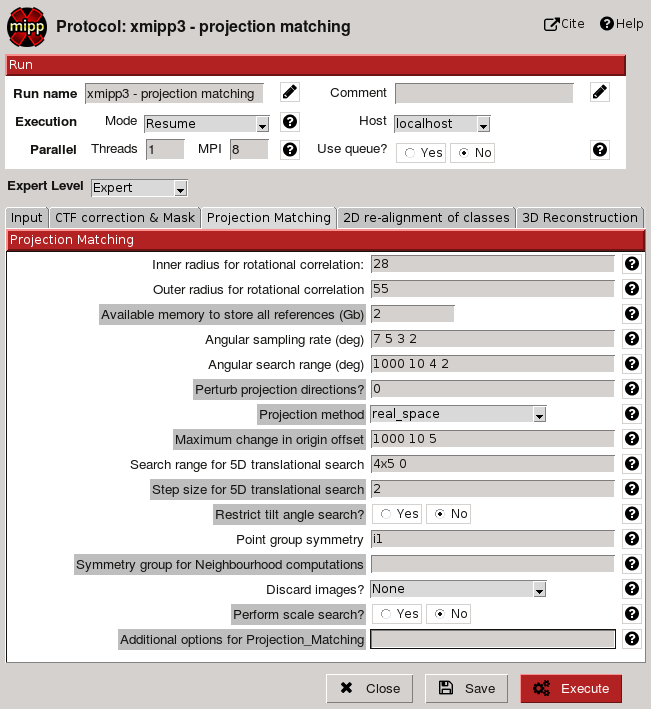
\includegraphics[width=0.75\textwidth]{{images/09.ProjMatchC}.png}
  \caption{Projection matching parameters III}
  \label{ProjMatchC}
 \end{figure}

  \begin{figure}
  \centering
  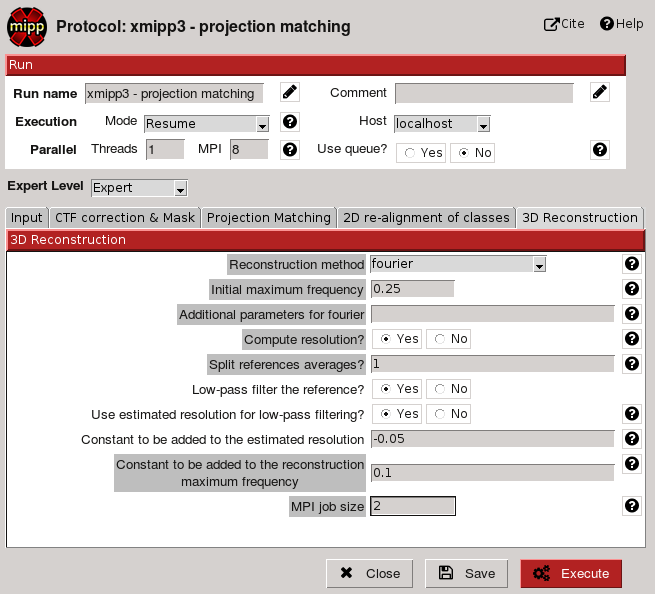
\includegraphics[width=0.75\textwidth]{{images/09.ProjMatchD}.png}
  \caption{Projection matching parameters IV}
  \label{ProjMatchD}
 \end{figure}

Finally, in order to visualize the obtained results click on
\textbf{Analyze Results} button. You will see a GUI as the one shown in
figure~\ref{ProjMatchViewer}.

 \begin{figure}
  \centering
  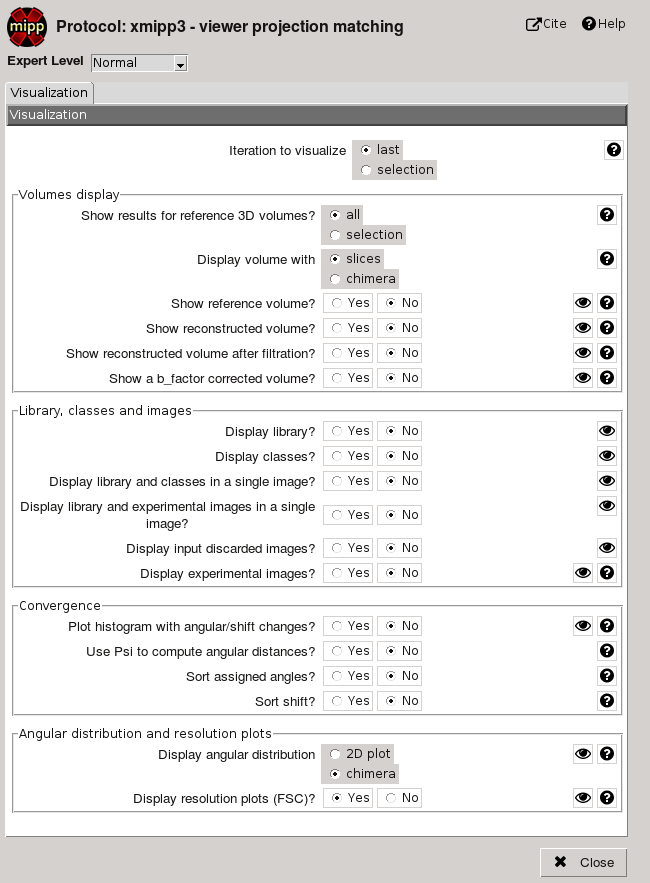
\includegraphics[width=0.75\textwidth]{{images/11.ProjMatchViewer}.png}
  \caption{Projection matching viewer}
  \label{ProjMatchViewer}
 \end{figure}

To see the volumes you can press \textbf{eye} button in the field
\textit{Display reconstructed volume?} and you will see the reconstructed
volume as shown in figure~\ref{volShowj} or in chimera if you select Chimera
checkbox (figure~\ref{volChimera}).

 \begin{figure}
  \centering
  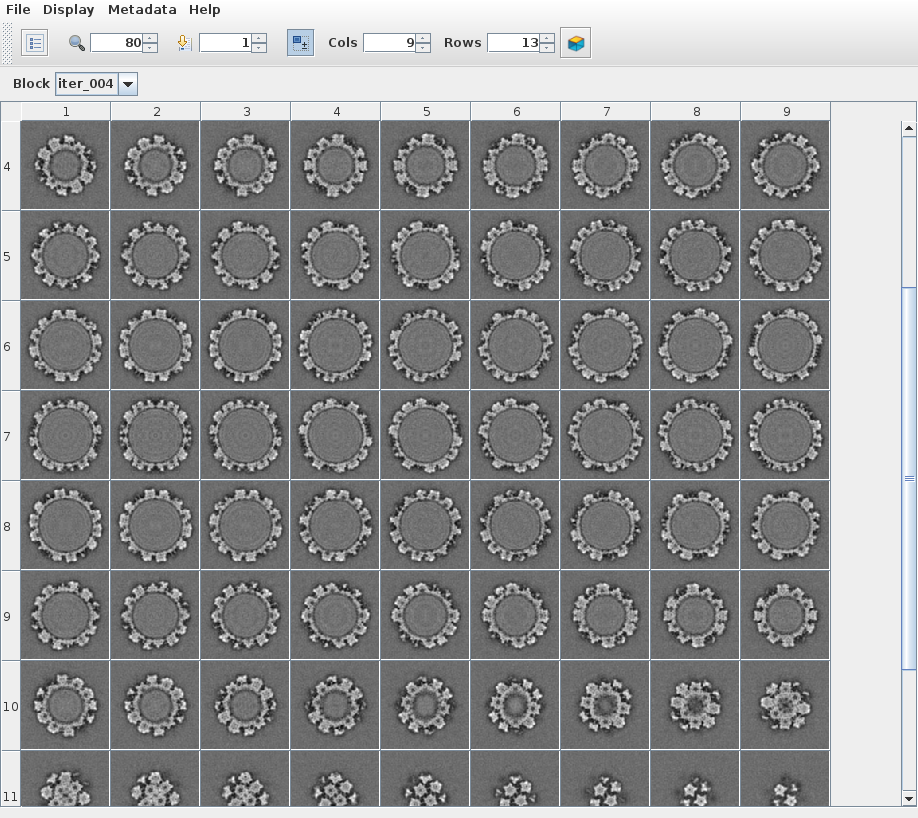
\includegraphics[width=0.75\textwidth]{{images/12.VolumeGalleries}.png}
  \caption{reconstructed volume}
  \label{volShowj}
 \end{figure}

 \begin{figure}
  \centering
  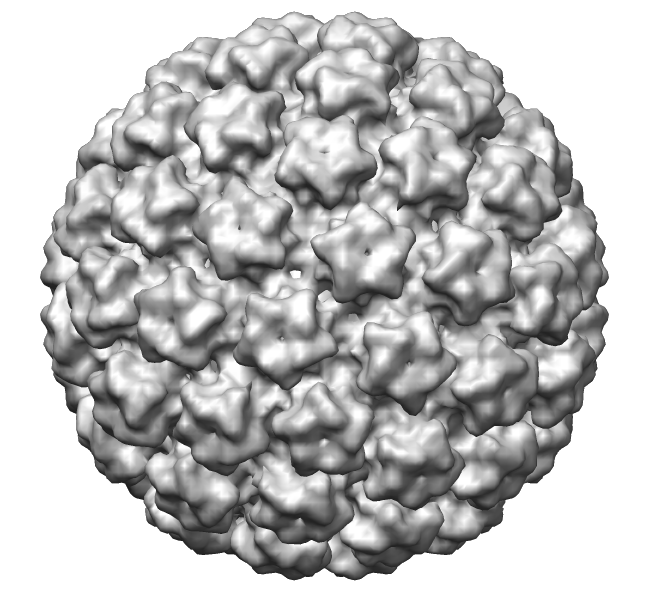
\includegraphics[width=0.75\textwidth]{{images/12.VolumeChimera}.png}
  \caption{reconstructed volume with chimera}
  \label{volChimera}
 \end{figure}

\subsection{Frealign refinement}

 If you want to refine the output volume of projection matching, you can
 use Frealign refinement protocol. First, you need the "same" SetOfParticles
 that has been processes with Projection matching, but with the features needed
 to Frealign.

 \begin{description}
  \item [Subset selection:]  To do this, the firs step is extract the particles
  again, but Preprocess tab changed as shown in figure~\ref{ExtractForFrealign}.
  
  \begin{figure}
   \centering
   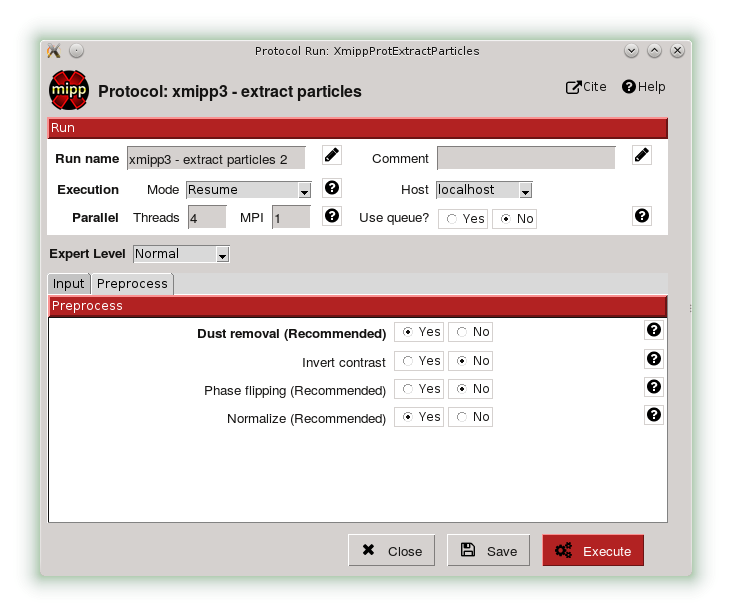
\includegraphics[width=0.75\textwidth]{{images/06.Extract_ParticlesC}.png}
   \caption{GUI of Extract Particles protocol II}
   \label{ExtractForFrealign}
 \end{figure}
 
 Once the particles are extracted, press on \textbf{Set operations $\rightarrow$ intersect sets}
 button. In first place, you set the last Extracted particles, and in second place
 the particles selected that has been used to refine a 3D reconstruction.
  \end{description}

 
The new SetOfParticles is the input of Frealign refinement protocol. Please, set the parameters
as shown in figures \ref{FrealignA}, \ref{FrealignB}, \ref{FrealignC} and \ref{FrealignD}

 \begin{figure}
  \centering
  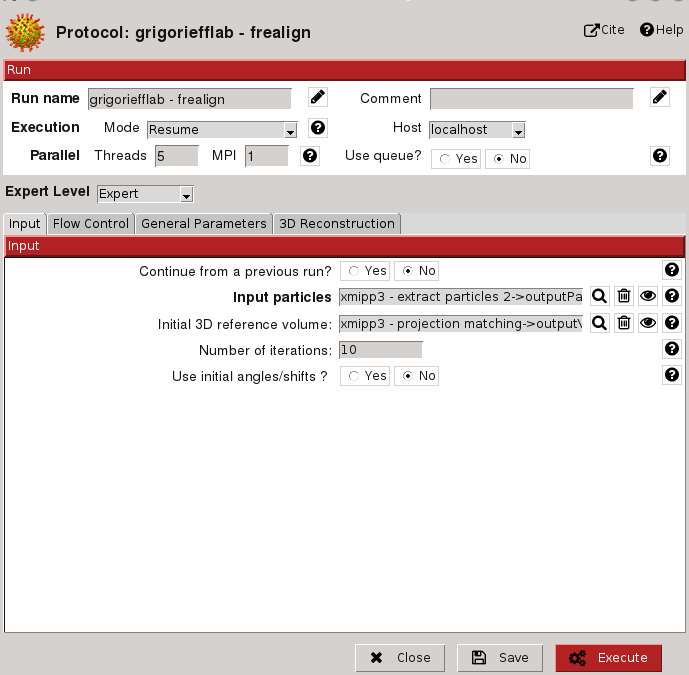
\includegraphics[width=0.75\textwidth]{{images/19.FrealignA}.png}
  \caption{Frealign parameters I}
  \label{FrealignA}
 \end{figure}

 \begin{figure}
  \centering
  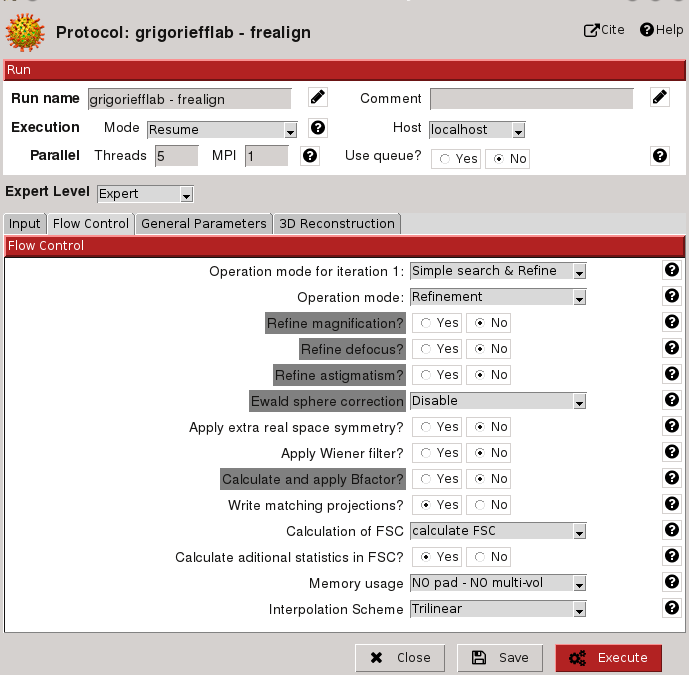
\includegraphics[width=0.75\textwidth]{{images/19.FrealignB}.png}
  \caption{Frealign parameters II}
  \label{FrealignB}
 \end{figure}

  \begin{figure}
  \centering
  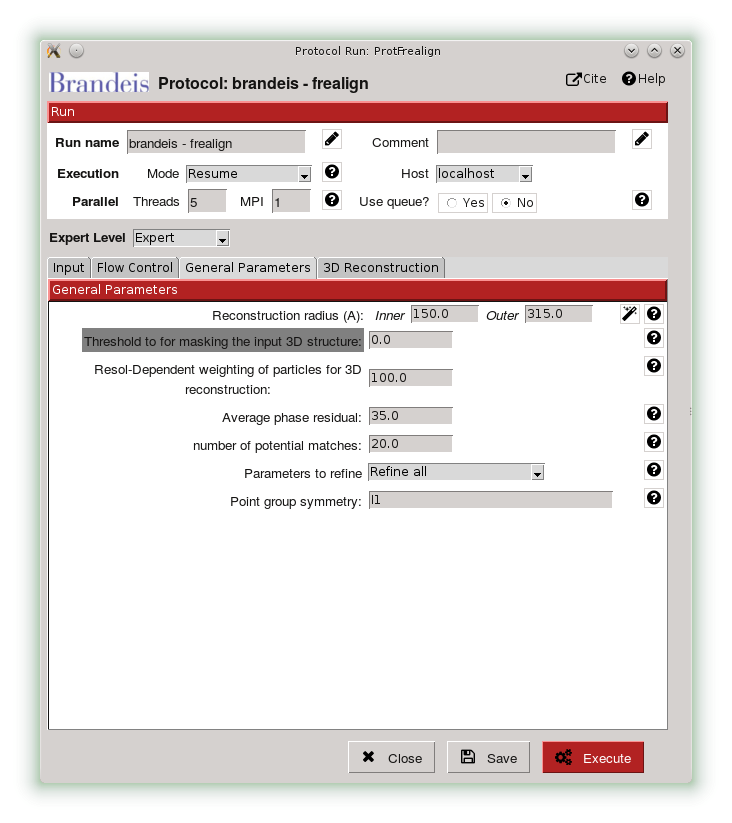
\includegraphics[width=0.75\textwidth]{{images/19.FrealignC}.png}
  \caption{Frealign parameters III}
  \label{FrealignC}
 \end{figure}

  \begin{figure}
  \centering
  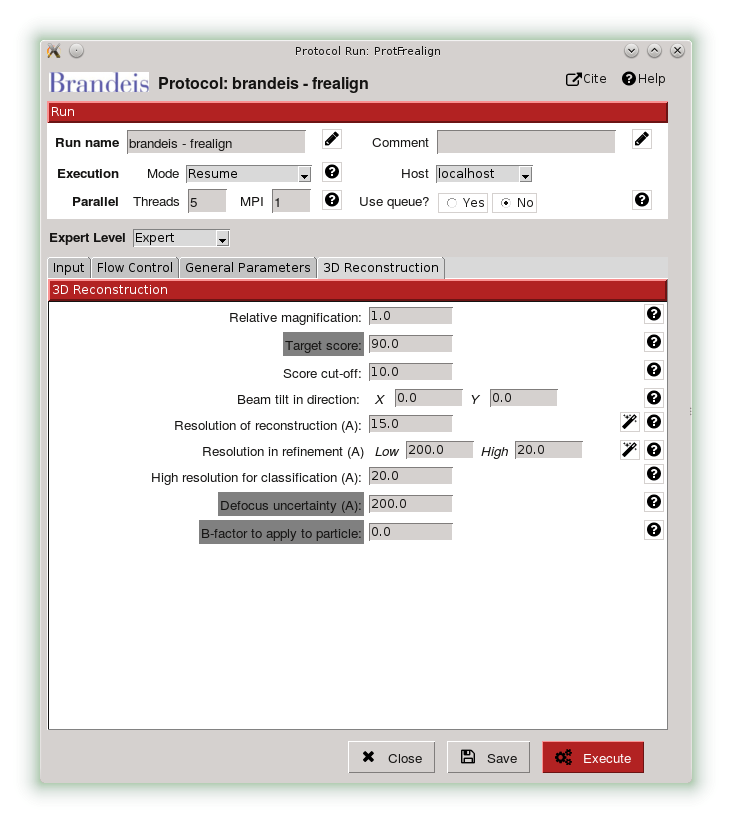
\includegraphics[width=0.75\textwidth]{{images/19.FrealignD}.png}
  \caption{Frealign parameters IV}
  \label{FrealignD}
 \end{figure}
 
Again, in order to visualize the obtained results click on
\textbf{Analyze Results} button. You will see a GUI as the one shown in
figure~\ref{FrealignViewer}.

 \begin{figure}
 \centering
 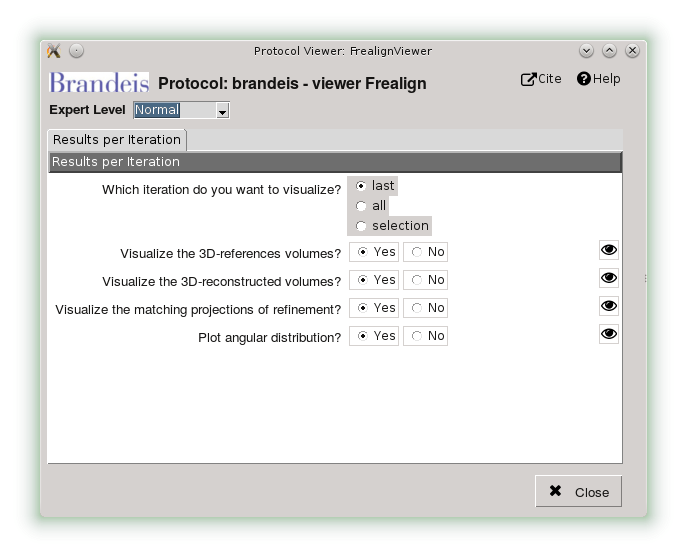
\includegraphics[width=0.75\textwidth]{{images/20.FrealignViewer}.png}
 \caption{Frealign viewer}
 \label{FrealignViewer}
 \end{figure}

\bibliographystyle{apalike}
\bibliography{../tutorial_common/em.bib}

\end{document}
